\section{Qualità di Processo}
Il gruppo \textit{DPCM 2077} ha deciso di seguire lo standard ISO/IEC/IEEE 12207:1995 per garantire la qualità del nostro progetto. Questo standard propone diversi processi, i quali sono stati scelti e adattati secondo le nostre esigenze. 
Il risultato sono i processi presentati di seguito.
	\subsection{Processi di sviluppo}
		\subsubsection{Sviluppo - Metriche}
		\paragraph{PROS: Percentuale di requisiti obbligatori soddisfatti}
		Indica la percentuale di requisiti obbligatori soddisfatti.
		\begin{itemize}
		\item espresso in percentuale: $PROS = \frac{requisiti \ obbligatori \ soddisfatti}{requisiti \ obbligatori \ totali}$;
		\item valore preferibile: 100\%;
		\item valore accettabile: 100\%.
		\end{itemize}
		
		\paragraph{CBO: Accoppiamento tra le classi di oggetti}
		Una classe è acccoppiata alla seconda se usa metodi o variabili definiti nella seconda.
		\begin{itemize}
		\item espresso con un valore intero: CBO;
		\item valore preferibile: $0 \leq CBO \leq 1$;
		\item valore accettabile: $0 \leq CBO \leq 6$.
		\end{itemize}
		
		\paragraph{Profondità della gerarchia}
		Misura la profondità del sito (numero di click necessari per arrivare all'informazione di interesse) in quanto un sito per essere di facile utilizzo non deve essere troppo profondo.
		\begin{itemize}
		\item misura: livello di profondità delle pagine;
		\item valore preferibile: $\leq 4$;
		\item valore accettabile: $ \leq 7$.
		\end{itemize}
		
		\paragraph{Numero di parametri per metodo}
		\begin{itemize}
		\item numero intero;
		\item valore preferibile: $\leq 3$;
		\item valore accettabile: $ \leq 4$.
		\end{itemize}
		
	\subsection{Processi organizzativi}
		\subsubsection{Gestione organizzativa - Metriche}
		\paragraph{BAC: Budget at Completion}
		Indica il budget totale allocato per il progetto.
		\begin{itemize}
		\item numero intero;
		\item valore preferibile: pari al preventivo;
		\item valore accettabile: il valore del preventivo con un errore massimo del $5\%$.
		\end{itemize}
		
		\paragraph{EV: Earned Value}
		Metrica di utilità per il calcolo di SV e CV. Costituisce il costo attribuibile al cliente se il progetto venisse interrotto alla data della misurazione.
		\begin{itemize}
		\item calcolo: $BAC \cdot \% \  di \ lavoro \ completato$;
		\item valore preferibile: $\geq 0$;
		\item valore accettabile: $\geq 0$.
		\end{itemize}
		
		\paragraph{PV: Planned Value}
		Metrica di utilità per il calcolo di SV e CV. Si tratta del valore del lavoro pianificato al momento del calcolo: denaro che si dovrebbe aver guadagnato in quel momento.
		\begin{itemize}
		\item calcolo: $BAC \cdot \% \ di \ lavoro \ pianificato$;
		\item valore preferibile: $\geq 0$;
		\item valore accettabile: $\geq 0$.
		\end{itemize}
		
		\paragraph{AC: Actual Cost}
		Il denaro speso fino al momento del calcolo.
		\begin{itemize}
		\item numero intero;
		\item valore preferibile: $0 \leq AC \le PV$;
		\item valore accettabile: $0 \leq AC \leq budget \ totale$.
		\end{itemize}
		
		\paragraph{SV: Schedule Variance}
		Esprime lo stato di anticipo o ritardo nello svolgimento del progetto rispetto alla pianificazione.
		\begin{itemize}
		\item calcolo: $SV = EV - PV$;
		\item valore preferibile: $\ge 0$;
		\item valore accettabile: $= 0$.
		\end{itemize}
		
		\paragraph{CV: Cost Variance}
		Differenza tra il costo del lavoro effettivamente completato e quello pianificato. Una CV positiva indica che si sta rispettando il budget.
		\begin{itemize}
		\item calcolo: $CV = EV - AC$
		\item valore preferibile: $\ge 0$;
		\item valore accettabile: $\geq 0$.
		\end{itemize}
		
	\subsection{Processi di supporto}
		\subsubsection{Verifica - Metriche}
		\paragraph{CC: Code Coverage}
		Indica il numero di righe di codice percorse dai test durante la loro esecuzione. Per linee di codice totali si intende tutte quelle appartenenti all'unità in fase di test.
		\begin{itemize}
		\item valore percentuale: $CC = \frac{linee \ di \ codice \ percorse}{linee \ di \ codice \ totali}$;
		\item valore preferibile: 100\%;
		\item valore accettabile: 80\%.
		\end{itemize}
		
		\subsubsection{Documentazione - Metriche}
		\paragraph{Indice di Gulpease}
		Indice della leggibilità del testo. Valuta la lunghezza delle parole e delle frasi rispetto al numero totale di lettere.
		\begin{itemize}
		\item valore intero da 0 a 100: $I = 89 + \frac{(300 \cdot numero \ di \ frasi - 10 \cdot numero \ di \ lettere)}{numero \ di \ parole}$;
		\item valore preferibile: $60 < I < 100$;
		\item valore accettabile: $40 < I < 100$.
		\end{itemize}
		
	\subsection{Tabella riassuntiva}
		\begin{center}
		\rowcolors{2}{white}{lightest-grayest}
		\begin{longtable}{|c|p{10cm}|c|}
			\hline
			\rowcolor{lighter-grayer}
			\textbf{Indice} & \textbf{Valore preferibile} & \textbf{Valore accettabile}  \\ 
						
			\hline
			\endhead
			
			\hline
			PROS & 100\% & 100\% \\
			\hline
			CBO & $0 \leq CBO \leq 1$ & $0 \leq CBO \leq 6$ \\
			\hline
			Profondità della gerarchia & $\leq 4$ & $\leq 7$ \\
			\hline
			Numero di parametri per metodo & $\leq 3$ & $\leq 4$ \\
			\hline
			BAC & pari al preventivo & il valore del preventivo con un errore massimo del $5\%$ \\
			\hline
			EV & $\geq 0$ & $\geq 0$ \\
			\hline
			PV & $\geq 0$ & $\geq 0$ \\			
			\hline
			AC & $0 \leq AC \le PV$ & $0 \leq AC \leq budget \ totale$ \\			
			\hline
			SV & $\ge 0$ & $= 0$ \\			
			\hline
			CV & $\ge 0$ & $\geq 0$ \\		
			\hline
			CC & 100\% & 80\% \\
			\hline
			Indice di Gulpease & $60 < I < 100$ & $40 < I < 100$ \\
			\hline
				
			\hiderowcolors
			\caption{Tabella dei test di sistema}		
		\end{longtable}	
	\end{center}
	
	\subsection{Grafici}
	\begin{figure}[H]
	\centering
	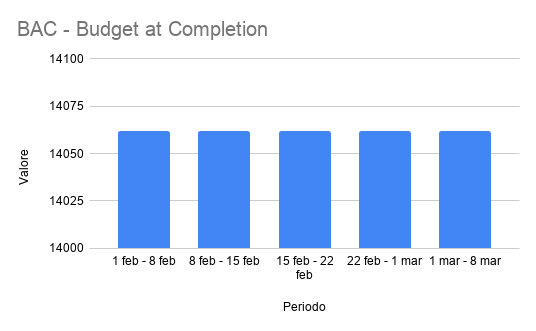
\includegraphics[width=0.7\linewidth]{res/images/BAC.png}
	\caption*{\textbf{Figura 1}: Grafico del BAC nel corso del periodo}
	\label{fig:Figura1}
\end{figure}

\begin{figure}[H]
	\centering
	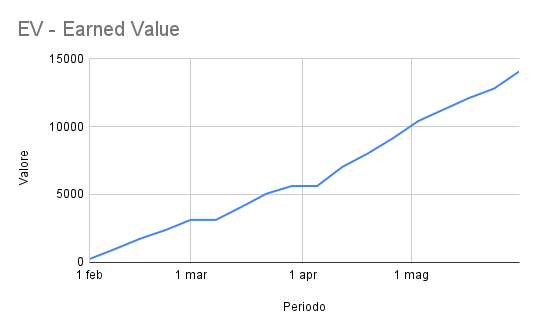
\includegraphics[width=0.7\linewidth]{res/images/EV.png}
	\caption*{\textbf{Figura 3}: Grafico del EV nel corso del periodo}
	\label{fig:Figura2}
\end{figure}

\begin{figure}[H]
	\centering
	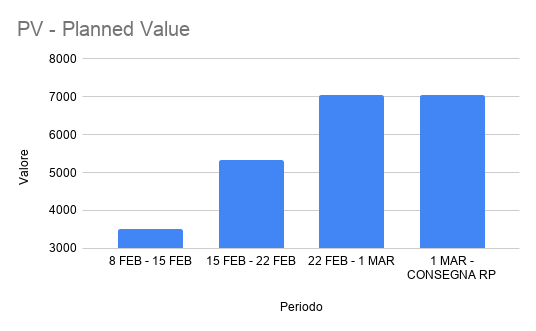
\includegraphics[width=0.7\linewidth]{res/images/PV.png}
	\caption*{\textbf{Figura 3}: Grafico del PV nel corso del periodo}
	\label{fig:Figura3}
\end{figure}
